\documentclass[a4paper,10pt]{article}
%\documentclass[a4paper,10pt]{scrartcl}

\usepackage[utf8]{inputenc}
\usepackage{hyperref}

\title{Floating Point Arithmetic Logic Unit}
\author{Suciu Andrei}
\date{October 2024}


\pdfinfo{%
  /Title    (Floating Point ALU)
  /Author   (Suciu Andrei)
  /Creator  ()
  /Producer ()
  /Subject  ()
  /Keywords ()
}



\usepackage{graphicx}
\usepackage{listings}
\usepackage{xcolor}
\graphicspath{ {images/} }

\definecolor{keywordsColor}{RGB}{101, 0, 153}
\lstset{
	language=VHDL,
	basicstyle=\ttfamily\footnotesize,
	keywordstyle=\color{keywordsColor}\bfseries,
	identifierstyle=\color{black},
	commentstyle=\color{gray},
	stringstyle=\color{green!60!black},
	numbers=left,
	numberstyle=\tiny\color{gray},
	stepnumber=1,
	tabsize=4,
	showstringspaces=false,
	breaklines=true,
	captionpos=b,
	frame=single,
	morekeywords={
		library, use, entity, architecture, signal, port, in, out, is, begin, end, std_logic, std_logic_vector,
		std_logic_1164, all, numeric_std, std_logic_arith, std_logic_unsigned, inout, to_integer, unsigned, signed,
		to_signed, to_unsigned
	}
}

\begin{document}
    \pagenumbering{gobble}
    \setlength{\parindent}{0pt}
    \begin{titlepage}
        \begin{center}
            \textbf{\large Department of Computer Science} \\[0.2cm]
            \textbf{\large Technical University of Cluj-Napoca} \\[0.5cm]
            
\includegraphics[width=1\textwidth]{utLogo.png} \\[1.0cm]

            \textbf{Floating Point Arithmetic Logic Unit} \\
            \textit{Laboratory activity 2024-2025} \\[4.0cm]

            Name: Suciu Andrei \\
            Group: 30431 \\
            Email: suciu.se.an@student.utcluj.ro\\

            \vfill

            Structure of Computer Systems\\[0.5cm]
            
\includegraphics[width=1\textwidth]{utLogo.png} \\[4.0cm]


        \end{center}
    \end{titlepage}
    \newpage

    \tableofcontents
    \newpage

    \pagenumbering{arabic}

    \section{Project Overview}
    \subsection{Specifications}
    Design an arithmetic logic unit on a 32-bit architecture capable of performing addition and multiplication operations on floating point numbers, encoded in the IEEE 754 standard. The ALU will be implemented on an FPGA, and must run and display various example operations.
    The ALU must be able to perform the following operations:
    \begin{itemize}
        \item 32-bit floating point addition
        \item 32-bit floating point multiplication
    \end{itemize}

    \subsection{Design}
    The implementation of the arithmetic logic unit will be designed in VHDL, using Vivado. The ALU will be contained within a master project which will provide the input and output display functionalities accoring to the FPGA provided at the laboratory. The project will be broken down into multiple smaller sources, each of which will be implemented using a behavioural style. Finally, all the project sources will be combined structurally to form a cohesive unit.

    \newpage

    \section{Bibliographic Research}
    \subsection{Arithmetic Logic Unit}
    In computing, an arithmetic logic unit (ALU) is a combinational digital circuit that is able to perform arithmetic on binary numbers. It is a fundamental building block of many other circuits, such as CPU or GPU.
    The ALU receives two input operands, an operation code, to decide which operation to perform, and optionally, a carry-in bit. Then, the result of the operation will be sent on the output signal.


    \subsection{Floating Point}
    In computing, numbers are represented in binary notation, as a series of bits, which can take values of either 1 or 0. In order to represent fractional parts, we must place a comma somewhere inside the number's representation. However, this greatly reduces the range of numbers which can be represented on a limitied amount of bits. In order to increase the range, we can imagine the comma moving (floating) left or right across the binary representation, according to what number we want to represent.

    Thus, we will to reserve a few bits for storing the position of the comma, creating a floating point number.

    \subsection{IEEE 754}
    The IEEE 754 defines the most widealy used standard for floating point numbers. Instead of storing the position of the comma, and the number itself, we will take advantage of scientific notation. In decimal scientific notation, the magnitude of the number is represented as a power of 10, and the "mantissa," essentially the core of the number, is stored as a fractional number between 1 and 10.

    Moving this format to binary, we can observe that no matter the number, the mantissa will always start with a leading "1." Thus, we can assume this part of the number and save 1 bit. The magnitude represents the exponent of a power of 2. Furthermore, there is one more bit for the sign of the number, 0 for positive, and 1 for negative.

    Overall, for a 32 bit number, the IEEE 754 standard formats the bits as such:
    \begin{itemize}
     \item 1 bit for the sign of the number
     \item 8 bits for the exponent
     \item 23 bits for the mantissa
    \end{itemize}

    \newpage
    \section{Development Plan}
    \subsection{Development Overview}
    It is proposed that by each project meeting a different subsection of the Floating Point ALU will be completed, to be tested at the laboratory, and any irregularities in behaviour to be elliminated. By the end of the semester, the whole project must be completed and must be presented by the last week.

    \subsection{Project Lab 1}
    The project overview and development plan will be finalised and presented.

    \subsection{Project Lab 2}
    The supporting environment for the project must be implemented and tested on the FPGA. It must be capable of displaying numbers stored in a Read-Only Memory using a Seven-Segment Display, and must be capable of switching between multiple display modes using switches or buttons as input.

    \subsection{Project Lab 3}
    The floating point addition subsection of the ALU must be implemented as a separate circuit and must be fully functional.

    \subsection{Project Lab 4}
    The floating point mutliplication subsection of the ALU must be implemented as a separate circuit and must be fully functional.

    \subsection{Project Lab 5}
    Any remaining part of the project will be implemented, and the board's functionality will be fully tested. Any errors in the circuit's operations will be removed. The documentation will be updated as well, should the need arise.

    \newpage
    \section{Floating Point ALU Structure}
    The FP ALU is composed of the three parts - the adder, the multiplier, and a multiplexer to change between them. The inputs are the two 32 bit IEEE-754 numbers, the operation to be performed, and a start bit to start the addition/multiplication.

    The outputs are the resulting number, and a bit to signal when the ALU is working and when the operation is over.


    \centerline{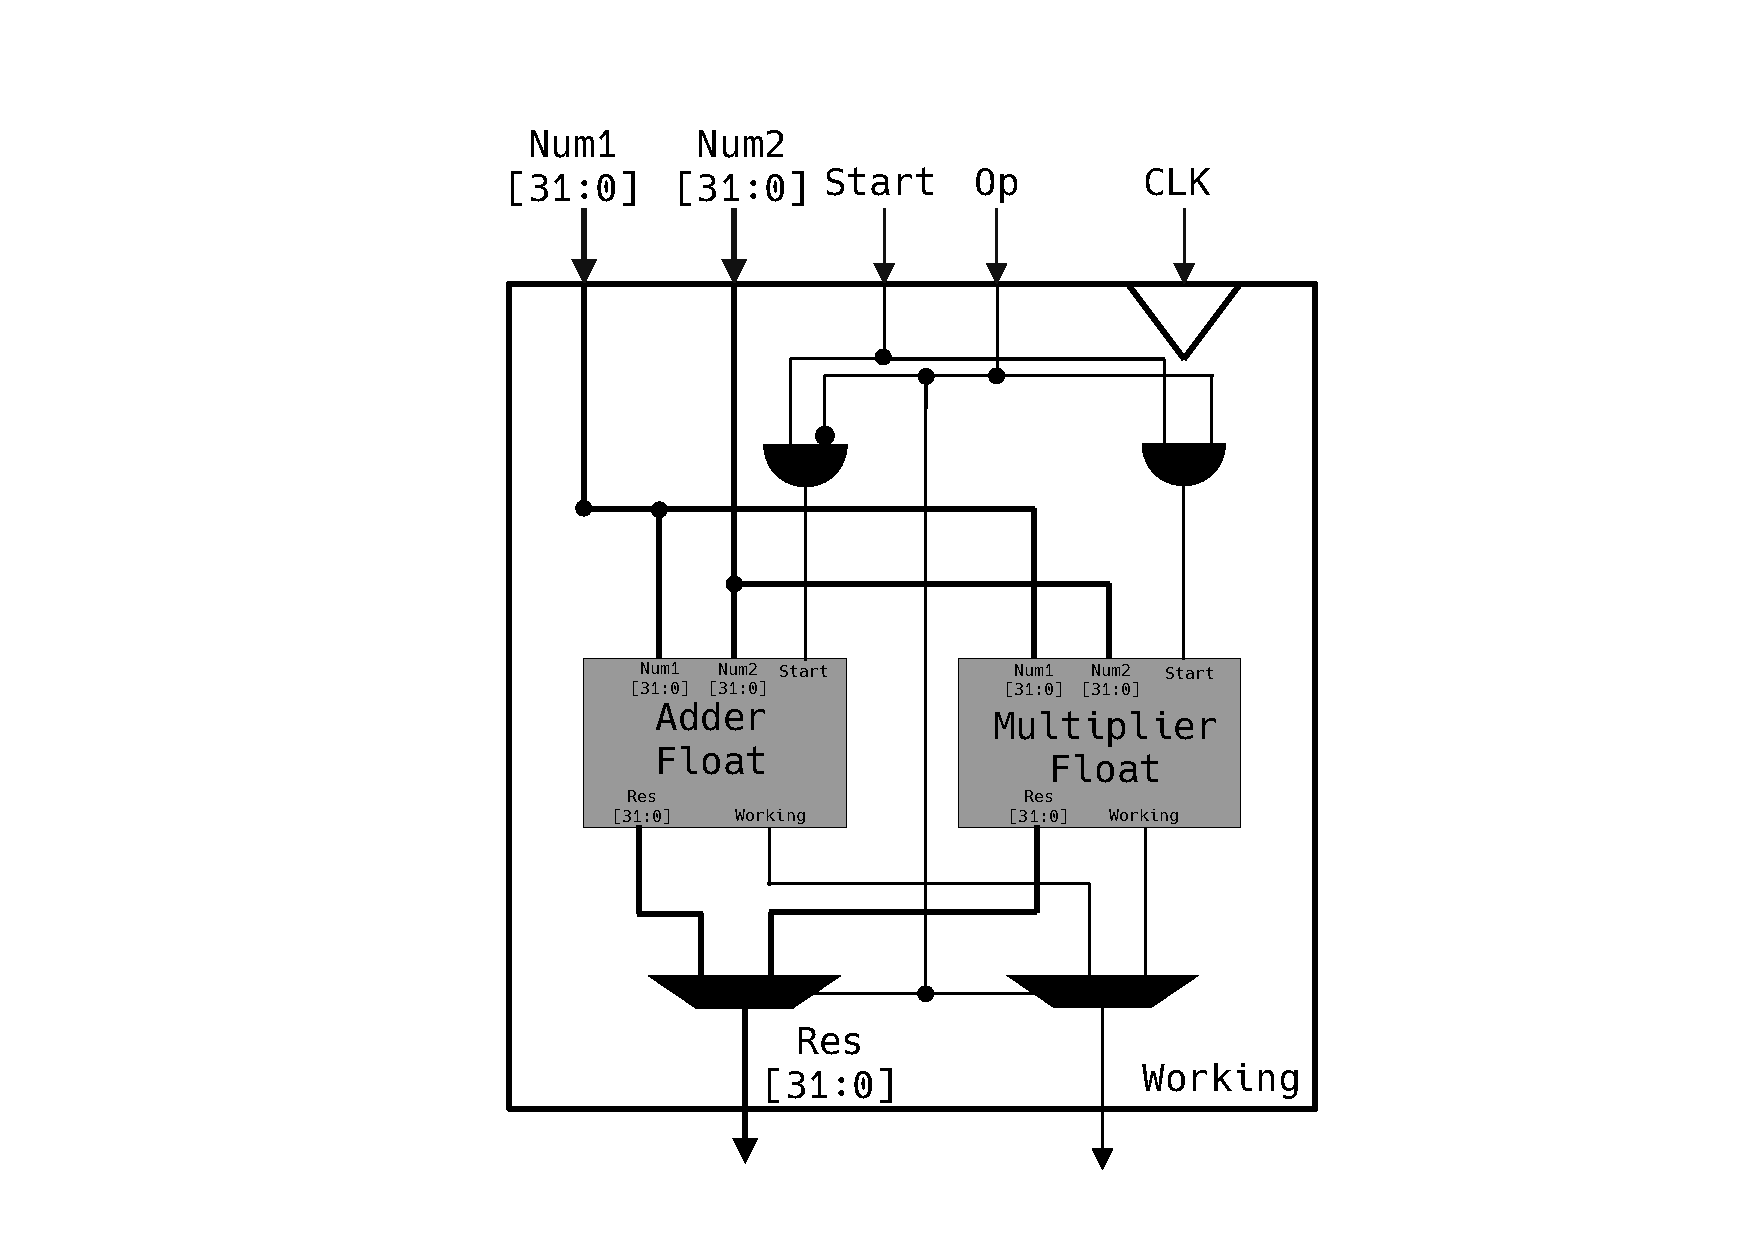
\includegraphics[scale=0.75]{ALUBig.pdf}}

    \newpage
    \section{Floating Point Adder}
    \subsection{Algorithm}
    The Floating point Adder takes as inputs the two numbers, A and B, which are divided into their respective sign, exponent, and mantissa (with a 1 implicitly placed on the 24th bit.

    First, we compare the exponents, and the mantissa of the number with the smaller exponent is shifted to the right and its exponent is incremented until the exponents are equal. This way, the numbers are aligned to the same exponent.

    Next, we perform the addition of the mantissa. If the signs are equal, we simply add the two mantissas together, otherwise, we subtract the smaller mantissa from the larger one, and use the sign of the number with the larger mantissa for the result.

    Finally, we realign the resulting number to the IEEE-754 standard. If the mantissa has become too large, and there is a '1' on the 25th bit, we shift the result right and increment the exponent. If the mantissa is too small, we shift left and decrement the exponent until there is a '1' on exactly the 24th bit.

    We also check for if the mantissa is equal to 0 and check for overflow and underflow of the exponent. If the mantissa is 0 or if we have an underflow of the exponent, we make the exponent and mantissa 0, so that there are only two values for the number 0. If there is an overflow of the exponent, we set the exponent to the maximum possible value and the mantissa to 0, for a standard infinity value.

    \newpage
    \subsection{Design}
    In order to implement the Floating Point Adder, we will use a 32 bit ALU, capable of addition, subtraction, incrementing, and decrementing. A comparator will also be needed which which can tell the greater number or whether they are equal. We will also use registers to store intermediate results, and a control unit to switch between the inputs and operations of the ALU.

    \centerline{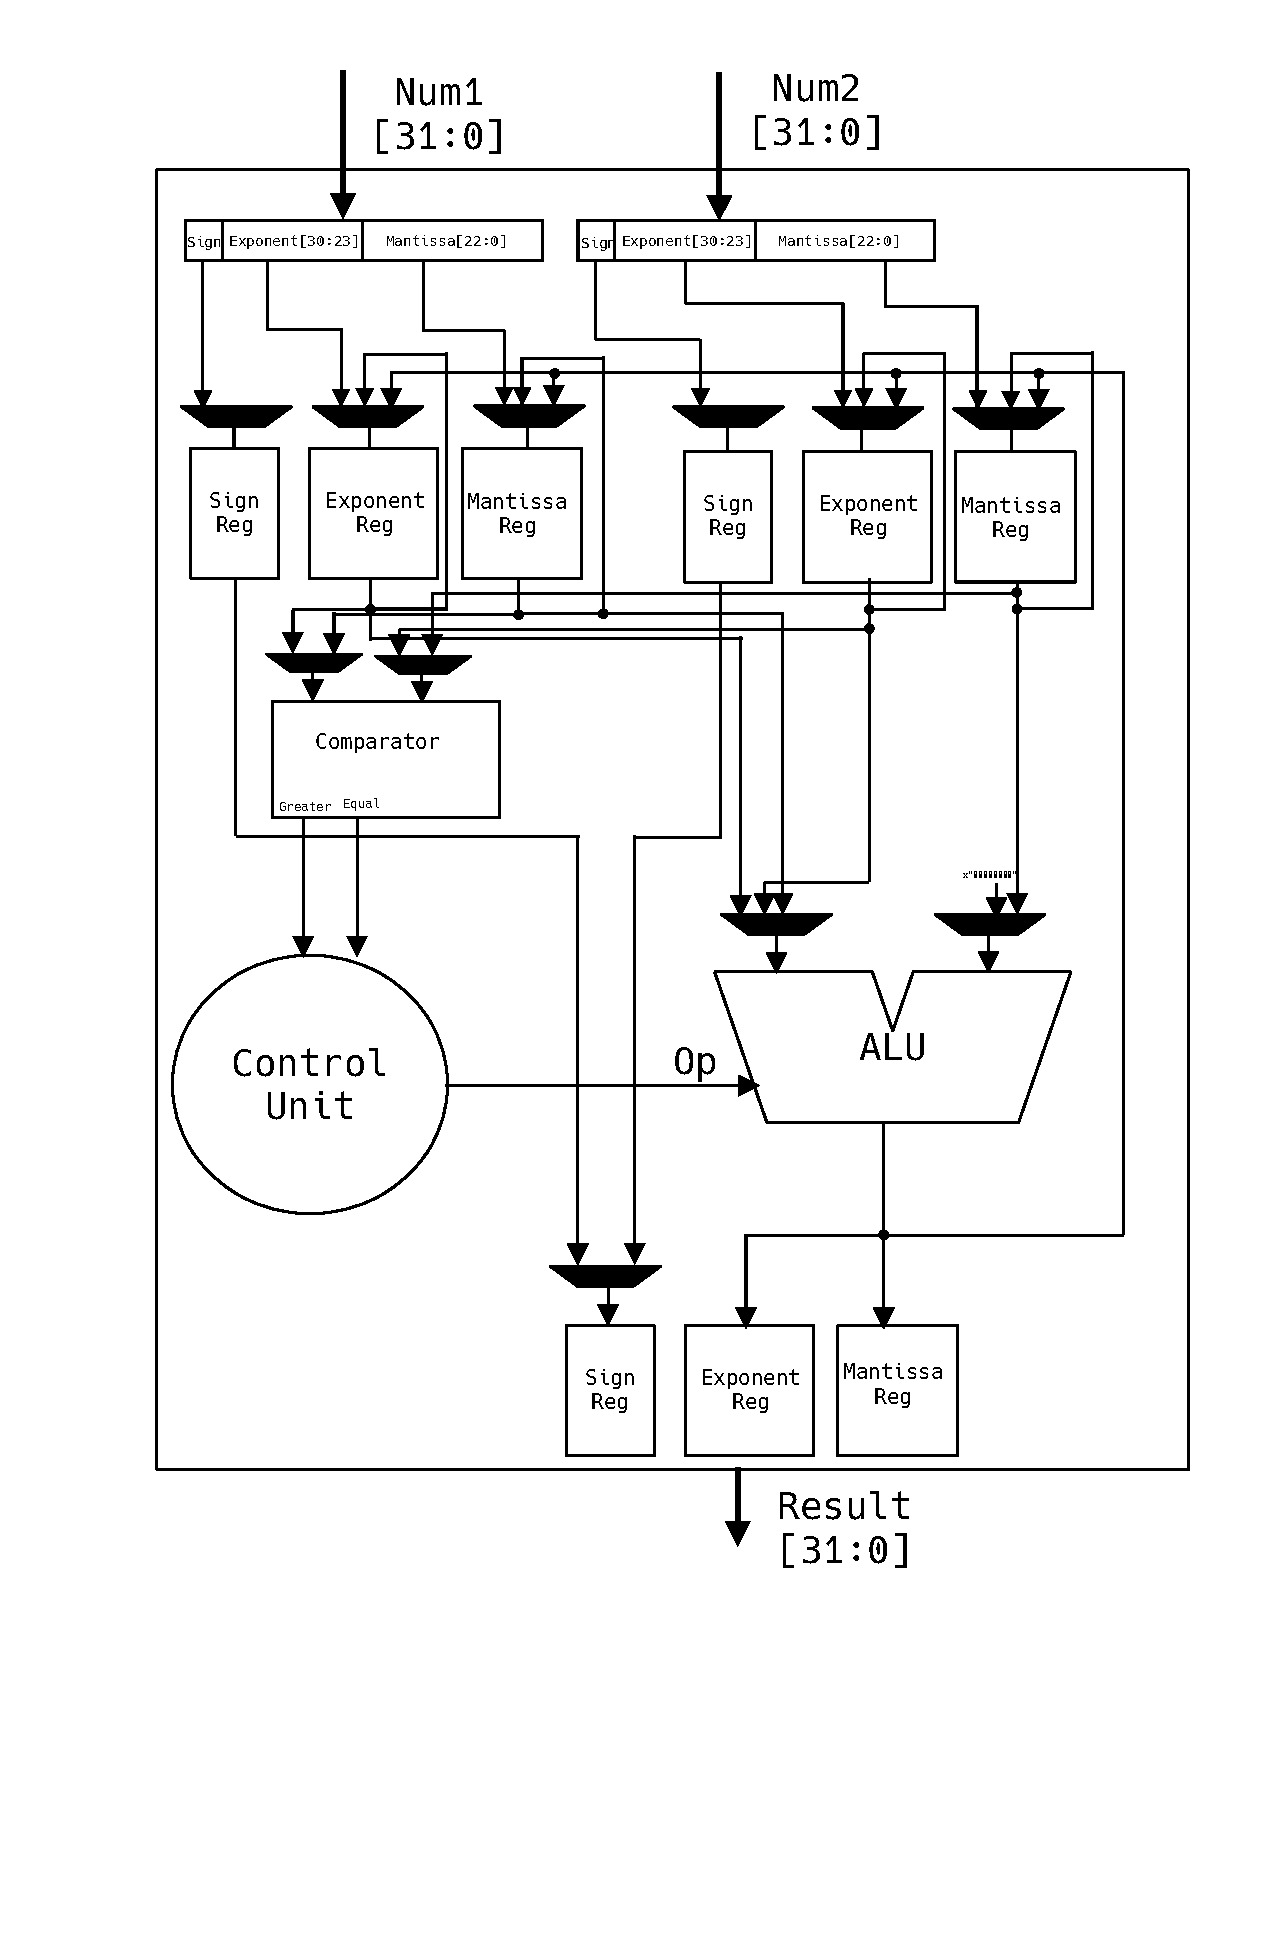
\includegraphics[scale=0.75, trim= 0cm 12cm 0cm 0cm]{adder.pdf}}

    \newpage
    \subsection{Implementation}
    The top level code was written in a structural style, while the simpler components were written behaviourally. Every component was implement separately to match the specifications mentioned above.\\
    \subsubsection{ALU}
    \centerline{\includegraphics[scale=0.75]{adderALU.pdf}}
    The ALU takes as input the two numbers, and a selection for which operation to be performed. Since it performs elementary operations, this is a combinational logic circuit, and requires no clock.\\
    The ouputs are the result of the operation, and an additional carry out bit, marked as \textit{cout}.\\
    The ALU is capable of performing four operations:
    \begin{itemize}
     \item Addition: \textit{result = numA + numB}
     \item Subtraction: \textit{result = numA - numB}
     \item Increment \textit{result = numA + 1}
     \item Decrement \textit{result = numA - 1}
    \end{itemize}
    In case of any overflow or underflow, the \textit{cout} bit is set to \textit{1}, otherwise it remains \textit{0}.\\
    \newpage
    \subsubsection{Comparator}
    The comparator takes as input two numbers, and the outputs \textit{eq} and \textit{greater} are set to $1$ if $numA > numB$ and if $numA = numB$ respectively.\\
    \centerline{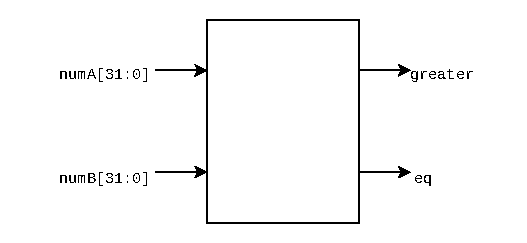
\includegraphics{comparator.pdf}}

    \subsubsection{Control Unit}
    The Control Unit is the most complex part of the floating point adder. It is a finite state machine which controls all the select signals for the various components of the design. It switches states synchronously, and based on the state and results from differing components, sets the select signals for the multiplexers, the write signals for the registers, and the operation for the ALU.

    The Control Unit is a finite state machine with five states:
    \begin{itemize}
      \item idle\_state:\\
      Machine is idle and not busy performing any operation.
      \item compare\_state:\\
      Compare the two exponents and shift the mantissa until they are equal.
      \item add\_state:\\
      Add the two mantissas together.
      \item align\_state:\\
      Realign the resulting number to match the IEEE-754 standard.
      \item verify\_overflow\_state:\\
      Check for overflow and write the corresponding result.
      \item verify\_underflow\_state:\\
      Check for underflow and write the corresponding result.
    \end{itemize}

    The entity for the floating point adder, and the components used is available \hyperref[sec:adder]{here}.



    \newpage
    \section{Floating Point Multiplier}
    \subsection{Algorithm}
    The Floating Point Multiplier takes as inputs the two numbers, A and B, which are divided into their respective sign, exponent, and mantissa (with a 1 implicitly placed on the 24th bit.

    First, we add the two exponents together and subtract 127 from the resulting sum. This is because the exponents are implicitly stored as (127 + exponent).

    Next, we perform the multiplication on the mantissas. We can use a Wallace Tree Multiplier to perform the multiplication in a single clock cycle, which simplifies the circuit significantly.

    Since we use a standard 32 bit Wallace Tree Multiplier and the mantissa has only 24 bits, we extend with zero to the right. The two mantissas will always start with a 1 on the MSB, and by multiplying them, the resulting number will also have a 1 on the 64th bit. We simply select the next most significatn 23 bits for the result mantissa, with no need to shift and align the number.

    Simmilarly to the adder, we apply the same standardisation steps for 0 or infinity. If the mantissa is 0, or there is an exponent underflow, we set all the exponent and mantissa bits to 0. If there is an exponent overflow, we set all exponent bits to 1, and all mantissa bits to 0.

    By using the steps described above, we can perform floating point multiplication in at most 5 clock cycles.

    \newpage
    \subsection{Design}
    In order to implement the Floating Point Multiplier, we will use a dedicated exponent adder to perform the exponent addition and subtracting 127, a 32 bit Wallace Tree Multiplier, and a Comparator. We also use registers to store intermediate values, and a control unit to give signals throughout the circuit.
    \centerline{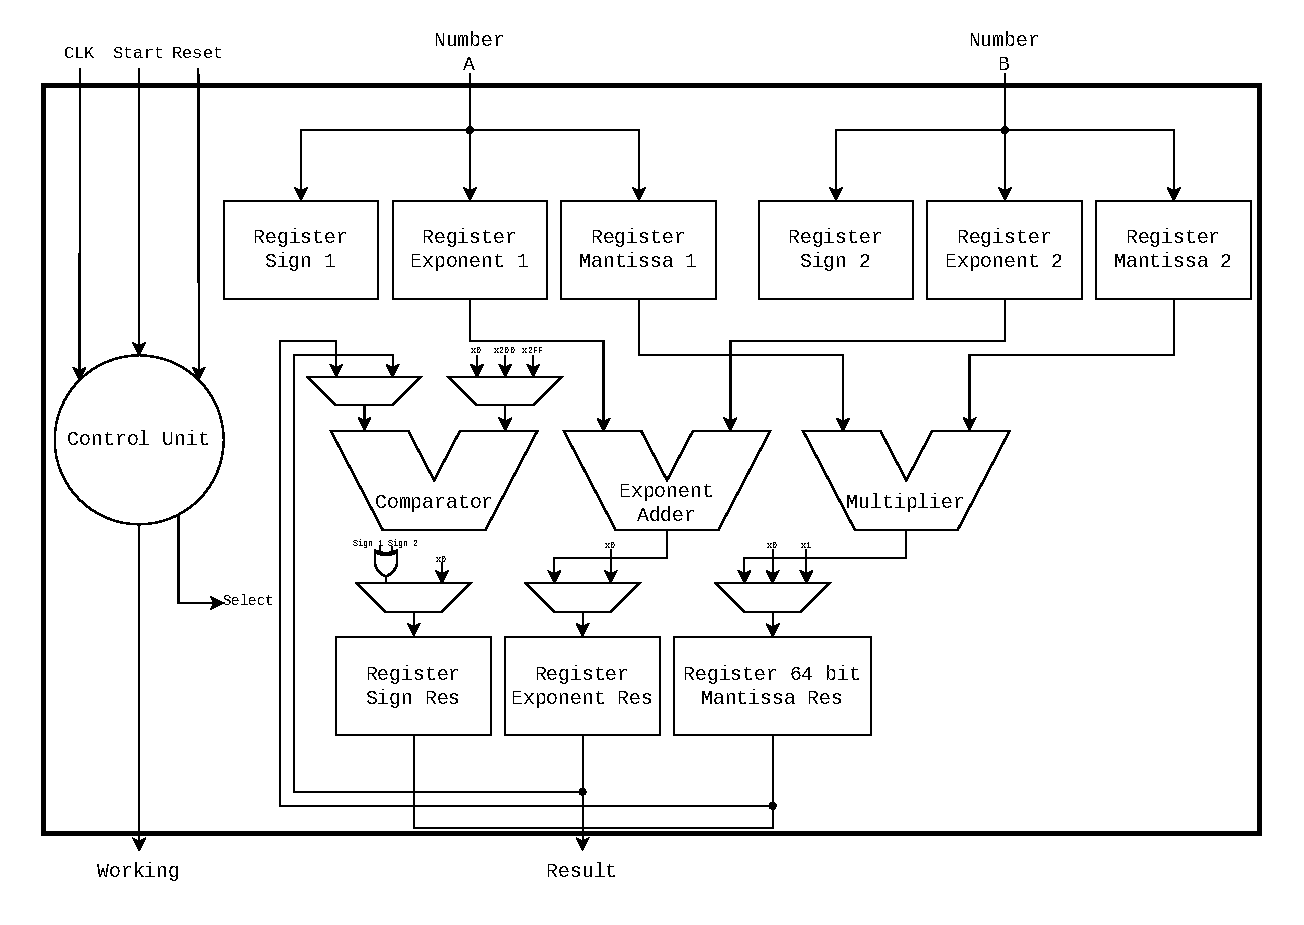
\includegraphics[scale=0.75, trim= 0cm 12cm 0cm 0cm]{fpMultiplier.pdf}}

    \newpage
    \subsection{Implementation}
    Simmilarly to the floating point adder, the top level was also written in a structural style, with the smaller components being written behaviourally.

    \subsubsection{Comparator}
    The comparator behaves the same as the one used for the adder, except it is capable of handling 64 bit numbers. It is used for checking the result for overflow or underflow in the final states of the process.

    \subsubsection{Exponent Adder}
    The exponent adder is a simple combinational logic circuit. It takes two 32 bit numbers, $exponent1$ and $exponent2$, and performs the operation\\
    \hspace*{1.0cm}$result <= exponent1 + exponent2 - 127$.

    \subsubsection{Multiplier}
    The mantissa multiplier was implemented as a wallace tree, capable of performing 32 bit multiplication. The result is on 64 bits. The desing was created recursively, starting from the 4 bit wallace tree multiplier. Each number is split into \textit{Low} and \textit{High}, and then multiplied, shifted, and added accordingly.
    \centerline{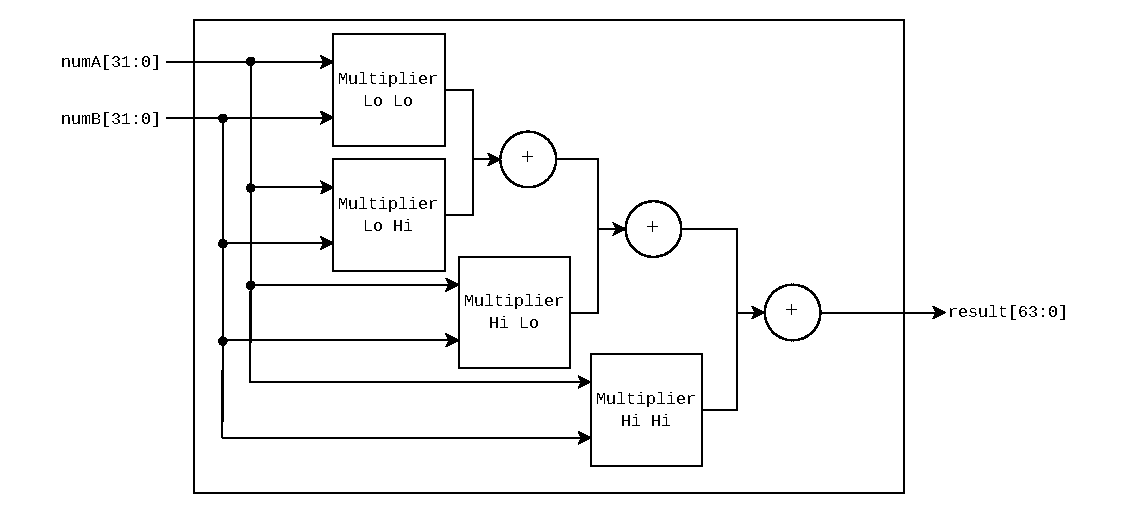
\includegraphics[scale=0.75]{multiplier.pdf}}

    \subsubsection{Control Unit}
    The Control Unit is similar to that of the floating point adder, though somewhat simpler. It is a finite state machine which controls all the select signals for the various components of the design. It switches states synchronously, and based on the state and results from differing components, sets just the select signals for the multiplexers and the write signals for the registers, with there being no operation signals.

    As oposed to the adder, which requires shifting the result an unknown amount of bits, the floating point multiplier will always complete the operation in at most 6 clock cycles.

    The Control Unit is a finite state machine with five states:
    \begin{itemize}
      \item idle\_state:\\
      Machine is idle and not busy performing any operation.
      \item add\_state:\\
      The exponent addition is performed\\
      $(exponentRes <= exponent1 + exponent2 - 127)$.
      \item multiply\_state:\\
      The two mantissas are multiplied together.
      \item align\_state:\\
      Realign the resulting number to match the IEEE-754 standard.
      \item verify\_overflow\_state:\\
      Check for overflow and write the corresponding result.
      \item verify\_underflow\_state:\\
      Check for underflow and write the corresponding result.
    \end{itemize}

    The entity for the floating point multiplier, and the components used is available \hyperref[sec:multiplier]{here}.


    \newpage
    \section{Code}
    \subsection{Floating Point Adder}
    \label{sec:adder}
    \subsubsection{Top level}
    \begin{lstlisting}
    entity adderFloat is
    Port ( clk : in STD_LOGIC;
           reset:in STD_LOGIC;
           start:in std_logic;
           num1:in std_logic_vector(31 downto 0);
           num2:in std_logic_vector(31 downto 0);
           res:out std_logic_vector(31 downto 0);
           dbState:out std_logic_vector(3 downto 0);
           working : out STD_LOGIC);
    end adderFloat;
    \end{lstlisting}

    \subsubsection{ALU}
    \begin{lstlisting}
    entity alu32bit is
    Port (
            numA : in STD_LOGIC_VECTOR (31 downto 0);
            numB : in STD_LOGIC_VECTOR (31 downto 0);
            op : in STD_LOGIC_vector(1 downto 0);
            output : out STD_LOGIC_VECTOR (31 downto 0);
            cout: out std_logic);
    end alu32bit;
    \end{lstlisting}

    \subsubsection{Comparator}
    \begin{lstlisting}
    entity comparator32bit is
    Port ( numA : in STD_LOGIC_vector(31 downto 0);
           numB : in STD_LOGIC_vector(31 downto 0);
           eq : out STD_LOGIC;
           greater : out STD_LOGIC);
    end comparator32bit;
    \end{lstlisting}

    \subsubsection{Control Unit}
    \begin{lstlisting}
    entity fpAdderControlUnit is
	Port (
		clk:in std_logic;
		reset:in std_logic;

		comparatorEq:in std_logic;
		comparatorGreater:in std_logic;

		outSign1_0:in std_logic;
		outSign2_0:in std_logic;
		outMantissaRes24:in std_logic;
		outMantissaRes23:in std_logic;

		start:in std_logic;

		writeSign1:out std_logic;
		writeSign2:out std_logic;
		writeSignRes:out std_logic;

		writeExponent1:out std_logic;
		writeExponent2:out std_logic;
		writeExponentRes:out std_logic;

		writeMantissa1:out std_logic;
		writeMantissa2:out std_logic;
		writeMantissaRes:out std_logic;

		selectSign1:out std_logic_vector(1 downto 0);
		selectExponent1:out std_logic_vector(1 downto 0);
		selectMantissa1:out std_logic_vector(1 downto 0);

		selectSign2:out std_logic_vector(1 downto 0);
		selectExponent2:out std_logic_vector(1 downto 0);
		selectMantissa2:out std_logic_vector(1 downto 0);

		selectSignRes:out std_logic_vector(1 downto 0);
		selectExponentRes:out std_logic_vector(1 downto 0);
		selectMantissaRes:out std_logic_vector(1 downto 0);

		dbState:out std_logic_vector(3 downto 0);
		working:out std_logic;

		comparatorSelect:out std_logic_vector(2 downto 0);
		alu32bitSelect:out std_logic_vector(2 downto 0);
		alu32bitOp:out std_logic_vector(1 downto 0)
	);
    end fpAdderControlUnit;
    \end{lstlisting}

    \subsubsection{Register with multiplexer}
    \begin{lstlisting}
     entity register32bitW4x1Mux is
    Port ( A : in STD_LOGIC_VECTOR (31 downto 0);
           B : in STD_LOGIC_VECTOR (31 downto 0);
           C : in STD_LOGIC_VECTOR (31 downto 0);
           D : in STD_LOGIC_VECTOR (31 downto 0);
           S: in std_logic_vector(1 downto 0);
           write : in STD_LOGIC;
           clk : in STD_LOGIC;
           output : out STD_LOGIC_VECTOR (31 downto 0));
    end register32bitW4x1Mux;
    \end{lstlisting}

    \newpage
    \subsection{Floating Point Multiplier}
    \label{sec:multiplier}
    \subsubsection{Top level}
    \begin{lstlisting}
    entity multiplierFloat is
    Port ( clk : in STD_LOGIC;
		   reset:in STD_LOGIC;
		   start:in std_logic;
		   num1:in std_logic_vector(31 downto 0);
		   num2:in std_logic_vector(31 downto 0);
		   res:out std_logic_vector(31 downto 0);
		   dbState:out std_logic_vector(3 downto 0);
		   working : out STD_LOGIC);
    end multiplierFloat;
    \end{lstlisting}

    \subsubsection{Exponent Adder}
    \begin{lstlisting}
    entity exponentAdder is
    Port ( exponent1 : in STD_LOGIC_VECTOR (31 downto 0);
           exponent2 : in STD_LOGIC_VECTOR (31 downto 0);
           result: out std_logic_vector(31 downto 0));
    end exponentAdder;
    \end{lstlisting}

    \subsubsection{Multiplier}
    \begin{lstlisting}
    entity multiplier32bit is
    Port ( numA : in STD_LOGIC_VECTOR (31 downto 0);
           numB : in STD_LOGIC_VECTOR (31 downto 0);
           result : out STD_LOGIC_VECTOR (63 downto 0));
    end multiplier32bit;
    \end{lstlisting}

    \subsubsection{Control Unit}
    \begin{lstlisting}
    entity fpMultiplierControlUnit is
	Port (
		clk:in std_logic;
		reset:in std_logic;

		comparatorEq:in std_logic;
		comparatorGreater:in std_logic;
		outMantissaRes63:in std_logic;

		start:in std_logic;

		writeSign1:out std_logic;
		writeSign2:out std_logic;
		writeSignRes:out std_logic;

		writeExponent1:out std_logic;
		writeExponent2:out std_logic;
		writeExponentRes:out std_logic;

		writeMantissa1:out std_logic;
		writeMantissa2:out std_logic;
		writeMantissaRes:out std_logic;

		selectSign1:out std_logic_vector(1 downto 0);
		selectExponent1:out std_logic_vector(1 downto 0);
		selectMantissa1:out std_logic_vector(1 downto 0);

		selectSign2:out std_logic_vector(1 downto 0);
		selectExponent2:out std_logic_vector(1 downto 0);
		selectMantissa2:out std_logic_vector(1 downto 0);

		selectSignRes:out std_logic_vector(1 downto 0);
		selectExponentRes:out std_logic_vector(1 downto 0);
		selectMantissaRes:out std_logic_vector(1 downto 0);

		dbState:out std_logic_vector(3 downto 0);
		working:out std_logic;
		comparatorSelect:out std_logic_vector(2 downto 0)
	);
    end fpMultiplierControlUnit;

    \end{lstlisting}

    \newpage
    \subsection{ALU Top level}
    \label{sec:aluTop}
    \begin{lstlisting}
    entity aluFloat is
    Port ( clk : in STD_LOGIC;
           num1 : in STD_LOGIC_VECTOR (31 downto 0);
           num2 : in STD_LOGIC_VECTOR (31 downto 0);
           op : in STD_LOGIC;
           start:in std_logic;
           res : out STD_LOGIC_VECTOR (31 downto 0);
           working:out std_logic);
    end aluFloat;
    \end{lstlisting}

    \newpage
    \section{Bibliography}
    \begin{thebibliography}{9}
      \bibitem{Steven Petryk}
        Steven Petryk,
        \href{https://www.youtube.com/watch?v=mKJiD2ZAlwM}{Adding IEEE-754 Floating Point Numbers},
        Oct 2015

      \bibitem{wikipediaFloat}
        Wikipedia,
        \href{https://en.wikipedia.org/wiki/IEEE_754}{IEEE 754},
        Oct 2024

      \bibitem{jan Misali}
        Jan Misali,
        \href{https://www.youtube.com/watch?v=dQhj5RGtag0}{how floating point works},
        May 2022
    \end{thebibliography}



\end{document}
